\documentclass{scrartcl}
\usepackage[utf8]{inputenc}
\usepackage{scrlayer-scrpage}
\usepackage[czech]{babel}
\usepackage{amsmath}
\usepackage{graphicx}

\cohead[Automaty a gramatiky]
        {Automaty a gramatiky}
\lohead[Úkol č. 1]
        {Úkol č. 1}
\rohead[Václav Luňák]
        {Václav Luňák}
\pagestyle{plain.scrheadings}

\graphicspath{ {.} }

\begin{document}
\section{Regularita jazyků}
\subsection{$L_1 = \{a^{2i} \vert i \in N_0 \}$}
Mějme následující automat:
\begin{center}
    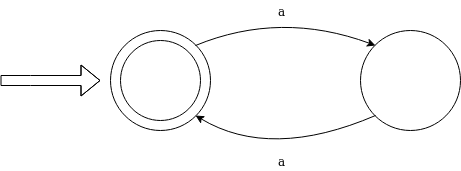
\includegraphics[width=250pt]{automat1.png}
\end{center}

Tento automat očividně přijímá právě slova sudé délky. Jazyk $L_1$ je tedy regulární.

\subsection{$L_2 = \{a^{i^2} \vert i \in N_0 \}$}

Mějme sporem $n$ z pumping lemmatu. Začneme se slovem $w = a^{n^2}$. Z lemmatu $w = xyz, \vert y \vert = s \geq 1, \vert xy \vert \leq n$. Definujme si pro $k \geq 0$ posloupnost $l_k = n^2 + (k-1)s$. \\

Kdyby jazyk $L_2$ byl regulární, musela by v něm být i slova všech délek $l_k$. Všimněme si, že $l_k$ tvoří rostoucí aritmetickou posloupnost s konstantní diferencí $s$. Délky slov ale musí být druhé mocniny, které aritmetickou řadu netvoří, neboť vzdálenost mezi nimi se lineárně zvětšuje ($(n+1)^2 - n^2 = 2n+1$). \\

Od určitého $n_0$ platí $2n+1 > s$ a tedy pro dostatečně velké $k$ najdeme $l_k, l_{k+1}$ příliš blízko u sebe na to, aby byla obě druhými mocninami. Alespoň jeden z členů tedy nepatří do jazyka, čímž máme spor s pumping lemmatem a důkaz, že $L_2$ není regulární.

\subsection{$L_3 = \{a^{2^i} \vert i \in N_0 \}$}

Mějme sporem $n$ z pumping lemmatu. Vezměme $w = a^{2^n} = xyz, \vert xy \vert \leq n, \vert y \vert = s \geq 1$. Opět z lemmatu musí jazyku náležet všechna slova délek $l_k = 2^n + (k-1)s$, což je opět rostoucí aritmetická posloupnost s diferencí $s$. \\

Stejně jako v předchozím případě pak vidíme, že rozdíl mezi délkami sousesdních slov roste s rostoucí délkou slova, jelikož $2^{n+1} - 2^n = 2^n$. Můžeme tedy opět najít dostatečně velké $k$ takové, že jedna z dvojice $l_k, l_{k+1}$ nemůže být mocninou dvojky, což nám dává spor s pumping lemmatem. Ani tento jazyk tedy není regulární.

\end{document}